\documentclass[aspectratio=169]{beamer}

\usetheme{numpex}

\usepackage{tikz,pgfplots,pgfplotstable}
\usepackage{tikz-shields}
\usepackage{booktabs}
\usepackage[scale=2]{ccicons}
\usepackage{minted}
\usepackage{tabularray}
\usepackage{currfile} % Required for getting the current file name
\newsavebox{\mintedbox}

\makeatletter
\newcommand\resetstackedplots{
\makeatletter
\pgfplots@stacked@isfirstplottrue
\makeatother
}

\definecolor{numpexblack}{RGB}{0,0,0}
\definecolor{numpexblue}{RGB}{42,46,128}
\definecolor{numpexfont}{RGB}{54,54,54}
\definecolor{numpexred}{RGB}{250,40,35}
\definecolor{numpexgray}{RGB}{127,127,127}
\definecolor{numpexlightgray}{RGB}{219,219,219}
\definecolor{numpexlightergray}{RGB}{237,237,237}


\usepackage[natbib, defernumbers=true, backend=biber, style=alphabetic, eprint=false, maxbibnames=1, url=false, doi=false]{biblatex}
\addbibresource{exa-ma.bib}


\title{Feelpp Apps}
\subtitle{Mini app to benchmark Feel++}
\date{15 September 2025}
\author{Thomas Saigre}
\institute{Cemosis, Université de Strasbourg}

\begin{document}

\maketitle


\section{Ingredients}

\begin{frame}
  \frametitle{Ingredients}

  We need:

  \begin{itemize}
    \item A program that runs some code (toolbox, ...)
    \item Input files (mesh, configuration files, ...)
    \item Quantities of interest to be monitored (error, time of execution, ...)
  \end{itemize}

\end{frame}


\begin{frame}
  \frametitle{Tool used: Feelpp-benchmarking}

  \begin{itemize}
    \item Tool to automate and facilitate the benchmarking process for applications.
    \item Available on GitHub: \githubBadge[baseline=2mm]{feelpp/benchmarking}
  \end{itemize}

\end{frame}


\begin{frame}
  \frametitle{Benchmarking Feel++ applications for NumPEx}

  \begin{itemize}
    \item Small applications for benchmarking usage of Feel++
    \item Development in \githubBadge[baseline=2mm]{numpex/apps-feelpp}
  \end{itemize}

  \pause

  Applications to be tested:
  \begin{small}
  \begin{itemize}
    \item \drawBadge[baseline=2mm,font=\tt, labelColor=green]{}{app-feelpp-discr} Solve a PDE with different discretization methods and order
    \item \drawBadge[baseline=2mm,font=\tt, labelColor=red]{}{app-feelpp-distance} Compute distance to a range of entities using FMM or BVH
    \item \drawBadge[baseline=2mm,font=\tt, labelColor=red]{}{app-feelpp-nlcrb} Test nonlinear compressive reduced basis methods
    \item \drawBadge[baseline=2mm,font=\tt, labelColor=orange]{}{app-feelpp-rb} Test reduced basis methods and empirical interpolation
    \item \drawBadge[baseline=2mm,font=\tt, labelColor=green!50!orange]{}{app-feelpp-io} Test I/O at large scale
  \end{itemize}
  \end{small}

\end{frame}


\begin{frame}[fragile]
  \frametitle{Example of benchmark configuration}

  \begin{lrbox}{\mintedbox}
  \RecustomVerbatimEnvironment{Verbatim}{BVerbatim}{}
  \begin{minted}[fontsize=\tiny, bgcolor=gray!10]{json}
{
  "executable": "build/default/src/app-feelpp-io/feelpp_app_io",
  "output_directory": "{{machine.output_app_dir}}/app-feelpp-io/io",
  "use_case_name": "eye-mesh",
  "timeout":"0-01:00:00",
  "input_file_dependencies":{
      "mesh_json":"mesh/{{parameters.mesh.value}}/Eye_Mesh3D_p{{parameters.resources.tasks.value}}.json",
      "mesh_hdf5":"mesh/{{parameters.mesh.value}}/Eye_Mesh3D_p{{parameters.resources.tasks.value}}.h5"
  },
  "options": [
    "--directory {{output_directory}}/{{instance}}/{{use_case_name}}",
    "--discretization {{parameters.discretization.value}}",
    "--repository.append.np 0",
    "--gmsh.filename mesh/{{parameters.mesh.value}}/Eye_Mesh3D_p{{parameters.resources.tasks.value}}.json"
  ],
}
  \end{minted}
  \end{lrbox}

  \resizebox{\textwidth}{!}{\usebox{\mintedbox}}

\end{frame}

\begin{frame}[fragile]
  \frametitle{Get the values for plotting}

  \begin{lrbox}{\mintedbox}
  \RecustomVerbatimEnvironment{Verbatim}{BVerbatim}{}
  \begin{minted}[fontsize=\tiny, bgcolor=gray!10]{json}
{
  "scalability": {
    "directory": "{{output_directory}}/{{instance}}/{{use_case_name}}",
    "clean_directory":true,
    "stages": [
      {
        "name": "timeMeasures",
        "filepath": "time_measures.json",
        "format": "json",
        "variables_path": "time.*",
        "units": { "*": "s"}
      }
    ]
  }
}
  \end{minted}
  \end{lrbox}

  \resizebox{\textwidth}{!}{\usebox{\mintedbox}}

\end{frame}

\begin{frame}[fragile]
  \frametitle{Bonus: a new feature in Feel++}

  Add any data to the journal during execution:

  \begin{minted}[bgcolor=gray!10]{cpp}
JournalManager::journalAdd( nl::json const &j, bool merge );
  \end{minted}

  Example:

  \begin{minted}[bgcolor=gray!10]{cpp}
tic();
offlineStage();
double offline_time = toc("offline");
nl::json time_tree = {{ "crb", {"offline", offline_time} }};
JournalManager::journalAdd( time_tree );
  \end{minted}



\end{frame}

\section{Benchmarks and results}


\begin{frame}{\texttt{app-feelpp-discr}}

\only<1-2>{
  \begin{columns}
  \begin{column}{0.4\textwidth}
      \begin{figure}
        \centering
        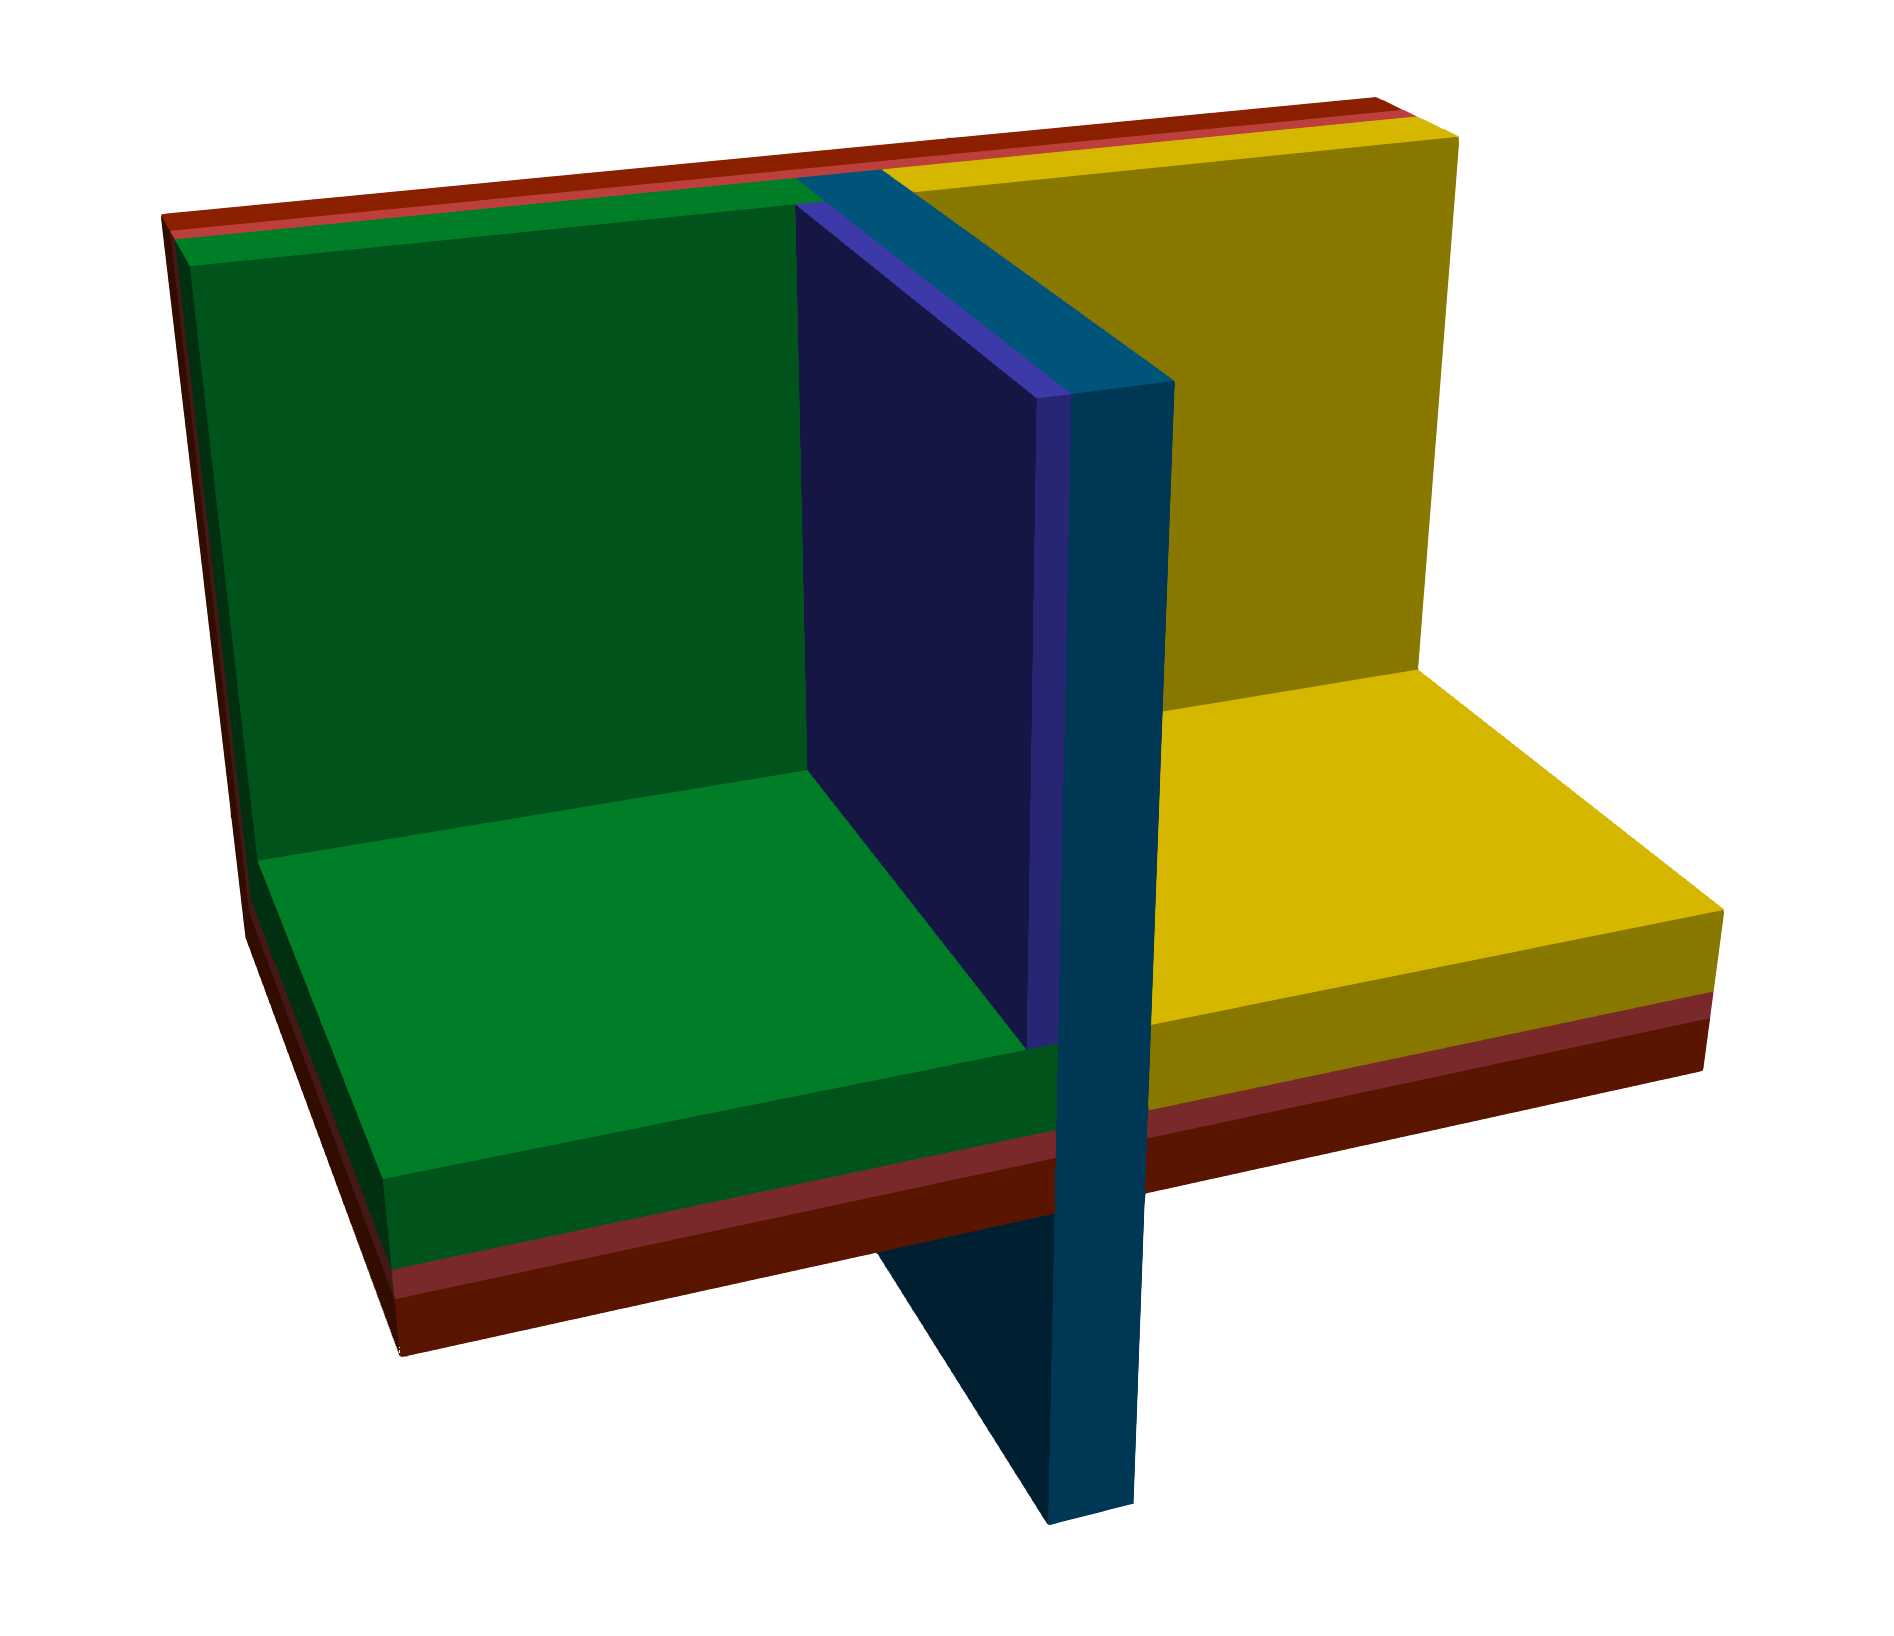
\includegraphics[width=\textwidth]{graphics/feelpp-benchmark-thermalbridges-geom.png}
      \end{figure}
  \end{column}

    \begin{column}{0.6\textwidth}
      \begin{itemize}
        \item Execution of the toolbox \emph{heat} on the thermal bridge benchmark\footfullcite{noauthor_iso_2017}.
        \item Execution for various mesh sizes, and order of discretization

        \pause

        \item To be added: Execution of the toolbox \emph{fluid} on the benchmark FDA
      \end{itemize}
  \end{column}

  \end{columns}
}

\only<3>{

\SetTblrInner{rowsep=0pt}
\begin{table}[!ht]
    \centering
    \resizebox{\textwidth}{!}{%
    \begin{tblr}{
        colspec={c*{7}{Q[c, cmd=\pgfmathprintnumber]}},
        vlines={numpexgray},
        hlines={numpexgray},
        row{1,2}={bg=numpexgray, fg=white, font=\bfseries, halign=c, cmd=\normalfont},
        rowhead=2, % This option excludes the first two rows from the column command
    }
    \SetCell[c=5]{c}{Mesh properties} & & & & & \SetCell[c=3]{c}{Number of degrees of freedom} & &\\
        Tag & \# points & \# edge & \# faces & \# elements & $P_1$ & $P_2$ & $P_3$ \\
        \texttt{M1} & 193654 & 1299920 & 2164759 & 1058492 & 193654 & 1493574 & 4958253\\
        \texttt{M2} & 1401135 & 9778744 & 16566803 & 8189193 & 1401135 & 11179879 & 37525426\\
        \texttt{M3} & 10572256 & 75307308 & 128722252 & 63987199 & 10572256 & 85879564 & 289909124\\
    \end{tblr}
    }

  \caption{Thermal bridges benchmarks - Statistics on meshes and number of degrees of freedom with respect to finite element approximation}
  \label{tab:wp1:feelpp:thermal_bridges:discr_stat}
\end{table}
}

\only<4>{
  % \documentclass[12pt]{article}

% \usepackage{pgf-pie}  % For pie charts
% \usepackage{currfile} % Required for getting the current file name
% \usepackage{tikz}     % Required for drawing graphics
% \usepackage{pgfplots}
% \usepackage{pgfplotstable}
% \pgfplotsset{compat=newest}
% \usepackage{underscore}

% \makeatletter
% \newcommand\resetstackedplots{
% \makeatletter
% \pgfplots@stacked@isfirstplottrue
% \makeatother
% }

% \begin{document}

\pgfplotstableread[col sep=comma]{\currfiledir/M2.csv}\dataA
\pgfplotstableread[col sep=comma]{\currfiledir/M3.csv}\dataB
\pgfplotstableread[col sep=comma]{\currfiledir/M4.csv}\dataC
\pgfplotstableread[col sep=comma]{\currfiledir/M5.csv}\dataD


\begin{figure}

  \begin{tikzpicture}[scale=0.7]
    \begin{axis}[
      width=\textwidth, height=0.6172\textwidth,
      xlabel={ Number of tasks }, ylabel={ execution time (s) },
      xticklabels from table={\dataA}{resources.tasks},
      xtick=data, xtick align=outside,
      ymajorgrids=true, yminorgrids=true,
      bar width=7pt,
      ybar stacked,
      legend style={at={(1.01,1)},anchor=north west}
    ]

      \addplot+[ybar, bar width=0.2,point meta=y,draw=black,fill=red ] table [x expr=\coordindex+0.25*1, y=Export] {\dataA} ;
      \addlegendentry{ LoadMesh }
      \addplot+[ybar, bar width=0.2,point meta=y,draw=black,fill=green ] table [x expr=\coordindex+0.25*1, y=CreateFunctionSpace] {\dataA} ;
      \addlegendentry{ CreateFunctionSpace }
      \addplot+[ybar, bar width=0.2,point meta=y,draw=black,fill=blue ] table [x expr=\coordindex+0.25*1, y=LoadMesh] {\dataA} ;
      \addlegendentry{ Export }
      \resetstackedplots
      \addplot+[ybar, bar width=0.2,point meta=y,draw=black,fill=red, forget plot ] table [x expr=\coordindex+0.25*2, y=Export] {\dataB} ;
      \addplot+[ybar, bar width=0.2,point meta=y,draw=black,fill=green, forget plot ] table [x expr=\coordindex+0.25*2, y=CreateFunctionSpace] {\dataB} ;
      \addplot+[ybar, bar width=0.2,point meta=y,draw=black,fill=blue, forget plot ] table [x expr=\coordindex+0.25*2, y=LoadMesh] {\dataB} ;
      \resetstackedplots
      \addplot+[ybar, bar width=0.2,point meta=y,draw=black,fill=red, forget plot ] table [x expr=\coordindex+0.25*3, y=Export] {\dataC} ;
      \addplot+[ybar, bar width=0.2,point meta=y,draw=black,fill=green, forget plot ] table [x expr=\coordindex+0.25*3, y=CreateFunctionSpace] {\dataC} ;
      \addplot+[ybar, bar width=0.2,point meta=y,draw=black,fill=blue, forget plot ] table [x expr=\coordindex+0.25*3, y=LoadMesh] {\dataC} ;
      \resetstackedplots
      \addplot+[ybar, bar width=0.2,point meta=y,draw=black,fill=red, forget plot ] table [x expr=\coordindex+0.25*4, y=Export] {\dataD} ;
      \addplot+[ybar, bar width=0.2,point meta=y,draw=black,fill=green, forget plot ] table [x expr=\coordindex+0.25*4, y=CreateFunctionSpace] {\dataD} ;
      \addplot+[ybar, bar width=0.2,point meta=y,draw=black,fill=blue, forget plot ] table [x expr=\coordindex+0.25*4, y=LoadMesh] {\dataD} ;

    \end{axis}
  \end{tikzpicture}

  \caption{ General Performance (P1) }
\end{figure}

% \end{document}
}


\end{frame}

\begin{frame}{\texttt{app-feelpp-rb}}

  \begin{itemize}
    \item Run the module of certified reduced basis of feelpp, on the test case of heat transfer in the human eyeball\footfullcite{saigre_model_2024}.
    \item Current state: the benchmark application run well, for a various number of parallel tasks, and on various meshes,
    \item but no figure has been generated yet :/
  \end{itemize}

\end{frame}


\begin{frame}
  \frametitle{\texttt{app-feelpp-io}}

  Small application that loads a mesh form disk, and write data on it.

  % \documentclass[12pt]{article}

% \usepackage{pgf-pie}  % For pie charts
% \usepackage{currfile} % Required for getting the current file name
% \usepackage{tikz}     % Required for drawing graphics
% \usepackage{pgfplots}
% \usepackage{pgfplotstable}
% \pgfplotsset{compat=newest}
% \usepackage{underscore}

% \makeatletter
% \newcommand\resetstackedplots{
% \makeatletter
% \pgfplots@stacked@isfirstplottrue
% \makeatother
% }

% \begin{document}

\pgfplotstableread[col sep=comma]{\currfiledir/M2.csv}\dataA
\pgfplotstableread[col sep=comma]{\currfiledir/M3.csv}\dataB
\pgfplotstableread[col sep=comma]{\currfiledir/M4.csv}\dataC
\pgfplotstableread[col sep=comma]{\currfiledir/M5.csv}\dataD


\begin{figure}

  \begin{tikzpicture}[scale=0.7]
    \begin{axis}[
      width=\textwidth, height=0.6172\textwidth,
      xlabel={ Number of tasks }, ylabel={ execution time (s) },
      xticklabels from table={\dataA}{resources.tasks},
      xtick=data, xtick align=outside,
      ymajorgrids=true, yminorgrids=true,
      bar width=7pt,
      ybar stacked,
      legend style={at={(1.01,1)},anchor=north west}
    ]

      \addplot+[ybar, bar width=0.2,point meta=y,draw=black,fill=red ] table [x expr=\coordindex+0.25*1, y=Export] {\dataA} ;
      \addlegendentry{ LoadMesh }
      \addplot+[ybar, bar width=0.2,point meta=y,draw=black,fill=green ] table [x expr=\coordindex+0.25*1, y=CreateFunctionSpace] {\dataA} ;
      \addlegendentry{ CreateFunctionSpace }
      \addplot+[ybar, bar width=0.2,point meta=y,draw=black,fill=blue ] table [x expr=\coordindex+0.25*1, y=LoadMesh] {\dataA} ;
      \addlegendentry{ Export }
      \resetstackedplots
      \addplot+[ybar, bar width=0.2,point meta=y,draw=black,fill=red, forget plot ] table [x expr=\coordindex+0.25*2, y=Export] {\dataB} ;
      \addplot+[ybar, bar width=0.2,point meta=y,draw=black,fill=green, forget plot ] table [x expr=\coordindex+0.25*2, y=CreateFunctionSpace] {\dataB} ;
      \addplot+[ybar, bar width=0.2,point meta=y,draw=black,fill=blue, forget plot ] table [x expr=\coordindex+0.25*2, y=LoadMesh] {\dataB} ;
      \resetstackedplots
      \addplot+[ybar, bar width=0.2,point meta=y,draw=black,fill=red, forget plot ] table [x expr=\coordindex+0.25*3, y=Export] {\dataC} ;
      \addplot+[ybar, bar width=0.2,point meta=y,draw=black,fill=green, forget plot ] table [x expr=\coordindex+0.25*3, y=CreateFunctionSpace] {\dataC} ;
      \addplot+[ybar, bar width=0.2,point meta=y,draw=black,fill=blue, forget plot ] table [x expr=\coordindex+0.25*3, y=LoadMesh] {\dataC} ;
      \resetstackedplots
      \addplot+[ybar, bar width=0.2,point meta=y,draw=black,fill=red, forget plot ] table [x expr=\coordindex+0.25*4, y=Export] {\dataD} ;
      \addplot+[ybar, bar width=0.2,point meta=y,draw=black,fill=green, forget plot ] table [x expr=\coordindex+0.25*4, y=CreateFunctionSpace] {\dataD} ;
      \addplot+[ybar, bar width=0.2,point meta=y,draw=black,fill=blue, forget plot ] table [x expr=\coordindex+0.25*4, y=LoadMesh] {\dataD} ;

    \end{axis}
  \end{tikzpicture}

  \caption{ General Performance (P1) }
\end{figure}

% \end{document}

\end{frame}


\section{Conclusion / Next steps}

\begin{frame}{Conclusion}

  \begin{itemize}
    \item Repository \texttt{apps-feelpp} to perform performance measures on the library Feel++,
    \item some applications already included, showing how the application behaves at different order and for various mesh sizes,
  \end{itemize}



  \pause

  \textbf{Next steps:}
  \begin{itemize}
    \item Trigger the run of benchmark from GitHub action,
    \item Add other benchmarks (FDA, ...) and applications (\emph{cf} above).
  \end{itemize}


\end{frame}

\end{document}
